%!TEX root = ../../book_ML.tex
\addtocontents{toc}{\protect\newpage}
\chapter{Bộ phân loại naive Bayes}
\label{cha:nbc}
\index{bộ phân loại naive Bayes -- naive Bayes classifier}
\index{NBC}

\section{Bộ phân loại naive Bayes}

Xét các bài toán phân loại với $C$ nhãn khác nhau. Thay vì tìm ra chính
xác nhãn của mỗi điểm dữ liệu $\bx \in \R^d$, ta có thể đi tìm xác suất để kết quả rơi vào mỗi nhãn:
\begin{math} 
\label{eqn:32_1}
p(y = c |\mathbf{x})
\end{math},
hoặc viết gọn thành $p(c|\mathbf{x})$. Biểu thức này được hiểu là xác suất để
đầu ra là nhãn $c$ biết rằng đầu vào là vector $\mathbf{x}$. Nếu tính được biểu thức này, ta có thể giúp xác định nhãn của mỗi điểm dữ liệu bằng cách chọn ra
nhãn có xác suất rơi vào cao nhất:
\begin{equation} 
\label{eqn:32_2}
c = \argmax_{c \in \{1, \dots, C\}} p(c | \mathbf{x}) 
\end{equation} 
Nhìn chung, khó có cách tính trực tiếp $p(c|\bx)$. Thay vào đó,
quy tắc Bayes thường được sử dụng:
\begin{align} 
  c =  \argmax_c p(c | \mathbf{x}) =  
  \argmax_c \frac{p(\mathbf{x} | c) p(c)}{p(\mathbf{x})} 
  =  \argmax_c p(\mathbf{x} | c) p(c) 
\end{align} 
Dấu bằng thứ hai xảy ra theo quy tắc Bayes, dấu bằng thứ ba xảy ra vì $p(\bx)$ ở
mẫu số không phụ thuộc vào $c$. Tiếp tục quan sát, $p(c)$ có thể được hiểu là
xác suất để một điểm \textit{bất kỳ} rơi vào nhãn $c$. Nếu tập huấn luyện lớn,
$p(c)$ có thể được xác định bằng phương pháp ước lượng hợp lý cực đại (MLE) -- là
tỉ lệ giữa số điểm thuộc nhãn $c$ và số điểm trong tập huấn luyện. Nếu tập huấn
luyện nhỏ, giá trị này có thể được xác định bằng phương pháp ước lượng hậu
nghiệm cực đại (MAP).
 
Thành phần còn lại $p(\mathbf{x} | c)$ là phân phối của các điểm dữ liệu trong
nhãn $c$. Thành phần này thường rất khó tính toán vì $\mathbf{x}$ là một biến
ngẫu nhiên nhiều chiều. Để có thể ước lượng được phân phối đó, tập huấn luyện
phải rất lớn. Nhằm đơn giản hoá việc tính toán, người ta thường giả sử
rằng các thành phần của biến ngẫu nhiên $\mathbf{x}$ độc lập với nhau khi đã
biết $c$:
\begin{equation} 
\label{eqn:32_6}
p(\mathbf{x} | c) = p(x_1, x_2, \dots, x_d | c) =  \prod_{i = 1}^d p(x_i | c)
\end{equation} 
Giả thiết các chiều của dữ liệu độc lập với nhau là quá chặt và trên thực tế, ít
khi tìm được dữ liệu mà các thành phần hoàn toàn độc lập với nhau. Tuy nhiên,
giả thiết \textit{ngây thơ} (\textit{naive}) này đôi khi mang lại những kết quả
tốt bất ngờ. Giả thiết về sự độc lập của các chiều dữ liệu này được gọi là
\textit{naive Bayes}. Một phương pháp xác định nhãn của dữ liệu dựa trên giả
thiết này có tên là \textit{phân loại naive Bayes (NBC)}.
 
Nhờ giả thiết độc lập, NCB có tốc độ huấn luyện và
kiểm tra rất nhanh. Việc này rất quan trọng trong các bài toán với dữ liệu lớn.
 
Ở bước huấn luyện, các phân phối $p(c)$ và $p(x_i | c), i = 1, \dots, d$ được xác định dựa vào dữ liệu huấn luyện. Việc xác định các giá trị này có thể được thực hiện bằng MLE hoặc MAP. 
 
Ở bước kiểm tra, nhãn của một điểm dữ liệu mới $\mathbf{x}$ được xác đinh bởi
\begin{equation} 
\label{eqn:32_7}
c = \argmax_{c \in \{1, \dots, C\}} p(c) \prod_{i=1}^d p(x_i | c).
\end{equation} 
Khi $d$ lớn và các xác suất nhỏ, biểu thức ở vế phải của~\eqref{eqn:32_7} là một
số rất nhỏ, khi tính toán có thể gặp sai số. Để giải quyết việc
này,~\eqref{eqn:32_7} thường được viết lại dưới dạng tương đương bằng cách lấy
$\log$ của vế phải:
\begin{equation} 
\label{eqn:32_7_1}
c = \argmax_{c \in \{1, \dots, C\}} \left(\log(p(c)) + \sum_{i=1}^d \log(p(x_i
| c))\right).
\end{equation} 
Việc này không ảnh hưởng tới kết quả vì $\log$ là một hàm đồng biến trên tập các số dương.  
 
Sự đơn giản của NBC mang lại hiệu quả đặc biệt trong các bài toán phân loại văn
bản, ví dụ bài toán lọc tin nhắn hoặc email rác. Trong phần sau của
chương này, chúng ta cùng xây dựng một bộ lọc email rác tiếng Anh đơn giản.
Cả quá trình huấn luyện và kiểm tra của NBC đều cực kỳ nhanh so với các phương
pháp phân loại phức tạp khác. Việc giả sử các thành phần trong dữ liệu là độc
lập với nhau khiến cho việc tính toán mỗi phân phối $p(\mathbf{x}_i|c)$ trở nên đơn giản.
 
% Mỗi giá trị $p(c), c = 1, 2, \dots, C$ có thể được xác định như là tần suất xuất
% hiện của class $c$ trong training data.
 
Việc tính toán $p(\mathbf{x}_i | c) $ phụ thuộc vào loại dữ liệu. Có ba loại
phân bố xác suất phổ biến là \textit{Gaussian naive Bayes},
\textit{multinomial naive Bayes}, và \textit{Bernoulli Naive}. Chúng ta cùng xem xét  từng loại.
 
 
 
 
 
\section{Các phân phối thường dùng trong NBC}
 
% \textit{Mục này chủ yếu được dịch từ \href{http://scikit-learn.org/dev/modules/naive_bayes.html#naive-bayes}{tài liệu của thư viện sklearn}.} 
 
\subsection{Gaussian naive Bayes }
\index{Gaussian naive Bayes}
Mô hình này được sử dụng chủ yếu trong loại dữ liệu mà các thành phần là các
biến liên tục. Với mỗi chiều dữ liệu $i$ và một nhãn $c$, $x_i$ tuân theo một
phân phối chuẩn có kỳ vọng $\mu_{ci}$ và phương sai $\sigma_{ci}^2$:
\begin{equation} 
\label{eqn:32_8}
p(x_i|c) = p(x_i | \mu_{ci}, \sigma_{ci}^2) =  \frac{1}{\sqrt{2\pi \sigma_{ci}^2}} \exp\left(- \frac{(x_i - \mu_{ci})^2}{2 \sigma_{ci}^2}\right)
\end{equation} 
Trong đó, bộ tham số $\theta = \{\mu_{ci}, \sigma_{ci}^2\}$ được xác định bằng
MLE\footnote{Xem ví dụ trang~\pageref{sssec:gassian_mle}.} dựa trên các điểm trong tập huấn luyện thuộc nhãn $c$.
% % \begin{equation} 
% % \label{eqn:32_9}
% % (\mu_{ci}, \sigma_{ci}^2) = \argmax_{(\mu_{ci}, \sigma_{ci}^2)} \prod_{n = 1}^N p(x_i^{(n)} \| \mu_{ci}, \sigma_{ci}^2)
% % \end{equation} 
% % ở đây $\$ 
% \textit{Đây là cách tính của thư viện sklearn. Chúng ta cũng có thể đánh giá các tham số bằng MAP nếu biết trước priors của $\mu_{ci}$ và $\sigma^2_{ci}$} 
 
 
\subsection{Multinomial naive Bayes }
\index{multinomial naive Bayes}

Mô hình này chủ yếu được sử dụng trong bài toán phân loại văn bản mà vector đặc
trưng được xây dựng dựa trên ý tưởng bag of words (BoW). Lúc này, mỗi văn bản
được biểu diễn bởi một vector có độ dài $d$ là số từ trong từ điển. Giá trị của
thành phần thứ $i$ trong mỗi vector là số lần từ thứ $i$ xuất hiện trong văn bản
đó. Khi đó, $p(x_i |c) $ tỉ lệ với tần suất từ thứ $i$ (hay đặc trưng thứ $i$
trong trường hợp tổng quát) xuất hiện trong các văn bản có nhãn $c$. Giá trị này
có thể được tính bởi
\begin{equation} 
\label{eqn:32_10}
\lambda_{ci} = p(x_i | c) = \frac{N_{ci}}{N_c}.
\end{equation} 
Trong đó: 
\begin{itemize}
    \item $N_{ci}$ là tổng số lần từ thứ $i$ xuất hiện trong các văn bản của
    nhãn $c$. Nó chính là tổng tất cả thành phần thứ $i$ của các
    vector đặc trưng ứng với nhãn $c$.
    
    \item $N_c$ là tổng số từ, kể cả lặp, xuất hiện trong nhãn $c$. Nói cách
    khác, $N_c$ là tổng độ dài của tất cả các văn bản thuộc nhãn $c$. Có
    thể suy ra rằng $N_c = \sum_{i = 1}^d N_{ci}$, từ đó $\sum_{i=1}^d
    \lambda_{ci} = 1$. 
\end{itemize}
 
\index{làm mềm Laplace -- Laplace smoothing}
Cách tính này có một hạn chế là nếu có một từ mới chưa bao giờ xuất hiện trong
nhãn $c$ thì biểu thức~\eqref{eqn:32_10} sẽ bằng không, dẫn đến vế phải
của~\eqref{eqn:32_7} bằng không bất kể các giá trị còn lại lớn thế nào (xem
thêm ví dụ ở mục sau). Để giải quyết việc này, một kỹ thuật được gọi là 
\textit{làm mềm Laplace} (Laplace smoothing) được áp dụng:
\begin{equation} 
\label{eqn:32_11}
\hat{\lambda}_{ci} = \frac{N_{ci} + \alpha}{N_{c} + d\alpha}
\end{equation} 
với $\alpha$ là một số dương, thường bằng 1, để tránh trường hợp tử số bằng
không. Mẫu số được cộng với $d\alpha$ để đảm bảo tổng xác suất $\sum_{i=1}^d
\hat{\lambda}_{ci} = 1$.
 Như vậy, mỗi nhãn $c$ được mô tả bởi một bộ các số dương có tổng bằng 1: $\hat{\lambda}_c = \{\hat{\lambda}_{c1}, \dots, \hat{\lambda}_{cd}\}$.
 
 
\subsection{Bernoulli Naive Bayes }
 
Mô hình này được áp dụng cho các loại dữ liệu mà mỗi thành phần là một giá trị
nhị phân -- bằng 0 hoặc 1. Ví dụ, cũng với loại văn bản nhưng thay vì đếm tổng
số lần xuất hiện của một từ trong văn bản, ta chỉ cần quan tâm từ đó có xuất
hiện hay không.
 
Khi đó, $p(x_i | c) $ được tính bởi
\begin{equation} 
p(x_i | c) = p(i | c)^{x_i}(1 - p(i | c) )^{1 - x_i}
\end{equation} 
với $p(i | c)$ được hiểu là xác suất từ thứ $i$ xuất hiện trong các văn
bản của class $c$, $x_i$ bằng 1 hoặc 0 tuỳ vào việc từ thứ $i$ có xuất hiện hay không.
 
 
 
\section{Ví dụ }
 
 
\subsection{Bắc hay Nam }
Giả sử trong tập huấn luyện có các văn bản d1, d2, d3, d4 như trong Bảng~\ref{tab:32_1}. Mỗi văn bản này thuộc vào một trong hai nhãn: B (\textit{Bắc}) hoặc N (\textit{Nam}). Hãy xác định nhãn của văn bản d5. 

\begin{table}[]
\centering
\caption{Ví dụ về nội dung của các văn bản trong bài toán Bắc hay Nam}
\label{tab:32_1}
\begin{tabular}{|l|c|l|c|}
\hline
                                & \textbf{Văn bản} & \textbf{Nội dung} & \textbf{Nhãn} \\ \hline \hline 
\multirow{4}{*}{Dữ liệu huấn luyện} & d1     & hanoi pho chaolong hanoi         & B   \\ \cline{2-4} 
                                & d2      & hanoi buncha pho omai         & B   \\ \cline{2-4} 
                                & d3      & pho banhgio omai         & B   \\ \cline{2-4} 
                                & d4      & saigon hutiu banhbo pho         & N   \\ \hline
Dữ liệu kiểm tra                        & d5      & hanoi hanoi buncha hutiu         & ?   \\ \hline
\end{tabular}
\end{table}

Ta có thể dự đoán rằng $\text{d5}$ có nhãn \textit{Bắc}.  
 
Bài toán này có thể được giải quyết bằng NBC sử dụng multinomial Naive Bayes
hoặc Bernoulli naive Bayes. Chúng ta sẽ cùng làm ví dụ với mô hình thứ nhất và
triển khai code cho cả hai mô hình. Việc mô hình nào tốt hơn phụ thuộc vào mỗi
bài toán. Ta có thể thử cả hai để chọn ra mô hình tốt hơn.
 
Nhận thấy rằng ở đây có hai nhãn B và N, ta cần đi tìm $p(\text{B})$ và $p(\text{N})$ dựa trên tần số xuất hiện của mỗi nhãn trong tập huấn luyện. Ta có
\begin{equation} 
\label{eqn:32_8}
p(\text{B}) = \frac{3}{4}, ~~~~~ p(\text{N}) = \frac{1}{4}.
\end{equation} 
Tập hợp toàn bộ các từ trong tập huấn luyện là 
$$V = \{\text{hanoi, pho, chaolong, buncha, omai, banhgio, saigon, hutiu, banhbo}\}$$ 
Tổng cộng số phần tử trong từ điển là $|V| = 9$.  
 
\begin{figure}[t]
\centering
    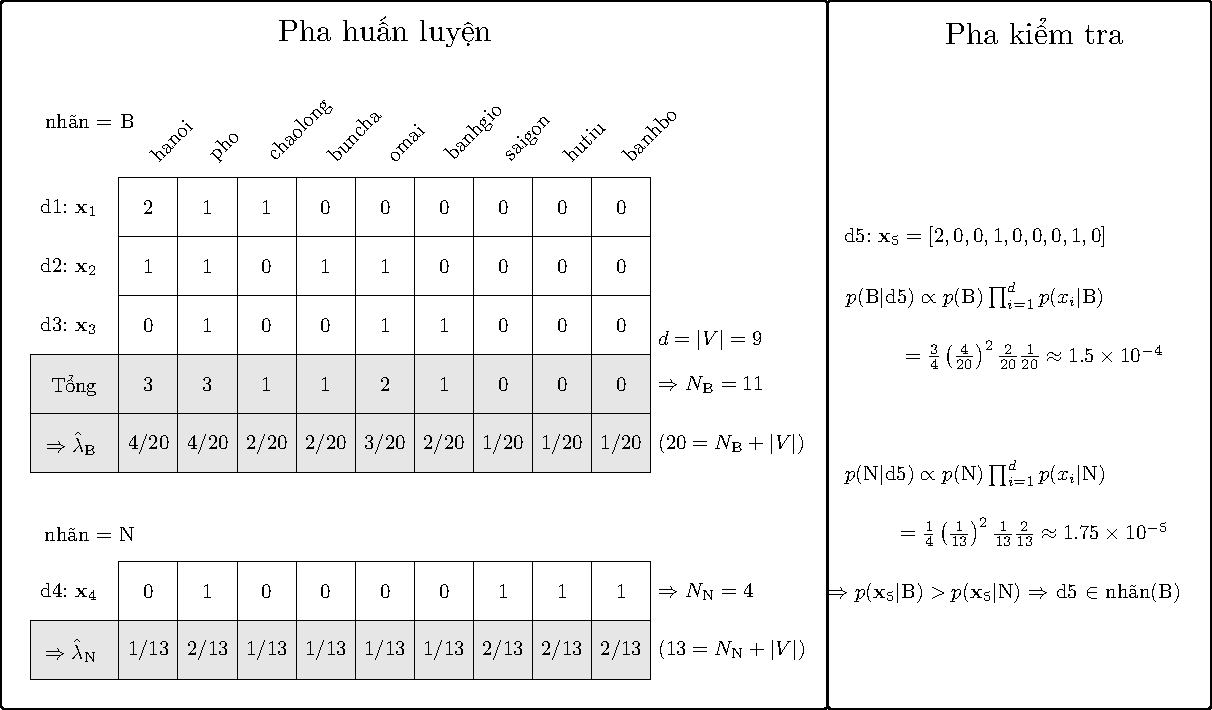
\includegraphics[width = \textwidth]{Chapters/03_SimpleML/32_nbc/latex/nbc.pdf}
    \caption[]{Minh hoạ NBC với Multinomial naive Bayes cho bài toán \textit{Bắc hay Nam}.}
    \label{fig:32_bn}
\end{figure}

Hình~\ref{fig:32_bn} minh hoạ quá trình huấn luyện và kiểm tra cho bài toán này
khi sử dụng Multinomial naive Bayes, trong đó làm mềm Laplace được sử dụng với
$\alpha = 1$. Chú ý, hai giá trị tìm được $1.5\times 10^{-4}$ và $1.75\times 10^{-5}$ không phải là hai xác suất cần tìm mà là hai đại lượng {tỉ lệ thuận} với hai xác suất đó. Để tính cụ thể, ta có thể làm như sau:
\begin{equation*} 
p(\text{B} | \text{d5}) = \frac{1.5\times 10^{-4}}{1.5\times 10^{-4} + 1.75\times 10^{-5}} \approx 0.8955, ~~~~ p(\text{N} | \text{d5}) = 1 - p(\text{B} | \text{d5}) \approx 0.1045. 
\end{equation*} 
Như vậy xác suất để d5 có nhãn B là 89.55\%, có nhãn N là 10.45\%. 
Bạn đọc có thể tự tính với ví dụ khác: $\text{d6 = pho hutiu banhbo}$. Nếu tính toán đúng, ta sẽ thu được  
\begin{equation*} 
p(\text{B} | \text{d6}) \approx 0.29, ~~~~ p(\text{N} | \text{d6}) \approx 0.71, 
\end{equation*} 
và suy ra $\text{d6}$ thuộc vào class N. 
 
\subsection{Bộ phân loại naive Bayes với thư viện scikit-learn}
 
Để kiểm tra lại các phép tính phía trên, chúng ta cùng giải quyết bài toán này bằng scikit-learn. Ở đây, dữ liệu huấn luyện và kiểm tra đã được đưa về dạng vector đặc trưng sử dụng BoW. 
\newpage  
\begin{lstlisting}[language=Python]
from __future__ import print_function 
from sklearn.naive_bayes import MultinomialNB 
import numpy as np  
# train data 
d1 = [2, 1, 1, 0, 0, 0, 0, 0, 0] 
d2 = [1, 1, 0, 1, 1, 0, 0, 0, 0] 
d3 = [0, 1, 0, 0, 1, 1, 0, 0, 0] 
d4 = [0, 1, 0, 0, 0, 0, 1, 1, 1] 
train_data = np.array([d1, d2, d3, d4]) 
label = np.array(['B', 'B', 'B', 'N'])  
# test data 
d5 = np.array([[2, 0, 0, 1, 0, 0, 0, 1, 0]]) 
d6 = np.array([[0, 1, 0, 0, 0, 0, 0, 1, 1]]) 
## call MultinomialNB 
model = MultinomialNB() 
# training  
model.fit(train_data, label) 

# test 
print('Predicting class of d5:', str(model.predict(d5)[0])) 
print('Probability of d6 in each class:', model.predict_proba(d6)) 
\end{lstlisting}
 \kq
\begin{lstlisting}
Predicting class of d5: B 
Probability of d6 in each class: [[ 0.29175335  0.70824665]] 
\end{lstlisting}
Kết quả này nhất quán với những kết quả được tính bằng tay ở trên. 
 
Nếu sử dụng Bernoulli naive Bayes, chúng ta cần thay đổi một chút về
feature vector. Lúc này, các giá trị khác không sẽ đều được đưa về một vì ta chỉ
quan tâm đến việc từ đó có xuất hiện trong văn bản hay không.
\begin{lstlisting}[language=Python]
from __future__ import print_function 
from sklearn.naive_bayes import BernoulliNB 
import numpy as np  
# train data 
d1 = [1, 1, 1, 0, 0, 0, 0, 0, 0] 
d2 = [1, 1, 0, 1, 1, 0, 0, 0, 0] 
d3 = [0, 1, 0, 0, 1, 1, 0, 0, 0] 
d4 = [0, 1, 0, 0, 0, 0, 1, 1, 1] 
train_data = np.array([d1, d2, d3, d4]) 
label = np.array(['B', 'B', 'B', 'N']) # 0 - B, 1 - N  
# test data 
d5 = np.array([[1, 0, 0, 1, 0, 0, 0, 1, 0]]) 
d6 = np.array([[0, 1, 0, 0, 0, 0, 0, 1, 1]]) 
## call MultinomialNB 
model = BernoulliNB() 
# training  
model.fit(train_data, label) 
# test 
print('Predicting class of d5:', str(model.predict(d5)[0])) 
print('Probability of d6 in each class:', model.predict_proba(d6)) 
\end{lstlisting}
\kq  
\begin{lstlisting}
Predicting class of d5: B 
Probability of d6 in each class: [[ 0.16948581  0.83051419]] 
\end{lstlisting}
 
Ta thấy rằng, với bài toán nhỏ này, cả hai mô hình đều cho kết quả giống nhau (xác suất tìm được khác nhau nhưng không ảnh hưởng tới quyết định cuối cùng).  
 
 
 
\subsection{Bộ phân loại naive Bayes cho bài toán lọc email rác}
% \index{spam filtering}
% \index{Ling-Spam dataset}
Tiếp theo, chúng ta cùng làm việc với một bộ cơ sở dữ liệu lớn hơn\footnote{Dữ liệu trong ví dụ này được lấy từ \textit{Exercise 6: Naive Bayes -- Machine Learning, Andrew Ng} (\url{https://goo.gl/kbzR3d}).}. Trong ví dụ này, dữ liệu đã được xử lý, và là một tập con của cơ sở dữ liệu \textit{Ling-Spam dataset} (\url{https://goo.gl/whHCd9}).  
 
 

% \index{stop word}
% \index{lemmatization}
% \index{non-word}
Tập dữ liệu này bao gồm 960 email tiếng Anh, được tách thành tập huấn luyện và tập kiểm tra theo tỉ lệ 700:260 với 50\% trong mỗi tập là các email rác.  

Dữ liệu ở đây đã được tiền xử lý. Các quy tắc xử lý như sau\footnote{sử dụng thư viện \textit{NLTK}
(\url{http://www.nltk.org/})}:
\begin{itemize}
    \item \textit{Loại bỏ \textit{stop words}}: Những từ xuất hiện thường xuyên như `and', `the', `of',... được loại bỏ vì chúng xuất hiện ở cả hai nhãn.

    \item \textit{Lemmatization}: Những từ có cùng gốc được đưa về cùng loại. Ví dụ, `include', `includes', `included' đều được đưa chung về `include'. Tất cả các từ cũng đã được đưa về dạng ký tự thường.
 
    
    \item \textit{Loại bỏ \textit{non-words}}: chữ số, dấu câu và các ký tự đặc biệt đã được loại bỏ.  
\end{itemize}


 
Dưới đây là một ví dụ của một email bình thường {trước khi được xử lý}:
 
\begin{lstlisting}
Subject: Re: 5.1344 Native speaker intuitions 
   
The discussion on native speaker intuitions has been extremely interesting, 
but I worry that my brief intervention may have muddied the waters. I 
take it that there are a number of separable issues. The first is the 
extent to which a native speaker is likely to judge a lexical string as 
grammatical or ungrammatical per se. The second is concerned with the 
relationships between syntax and interpretation (although even here the 
distinction may not be entirely clear cut). \end{lstlisting}
 
\newpage 
và {sau khi được xử lý}:
 
\begin{lstlisting}[language=Python]
re native speaker intuition discussion native speaker intuition extremely  
interest worry brief intervention muddy waters number separable issue first  
extent native speaker likely judge lexical string grammatical ungrammatical  
per se second concern relationship between syntax interpretation although  
even here distinction entirely clear cut  
\end{lstlisting}
 
Dưới đây là một ví dụ về {email rác sau khi được xử lý}:
 
\begin{lstlisting}
financial freedom follow financial freedom work ethic extraordinary desire 
earn least per month work home special skills experience required train 
personal support need ensure success legitimate homebased income opportunity 
put back control finance life ve try opportunity past fail live promise
\end{lstlisting}
 
Các từ `financial',
`extraordinary', `earn', `opportunity',... là những từ thường thấy trong các email rác.
 
Trong ví dụ này, chúng ta sẽ sử dụng multinomial naive Bayes. 
 
Để bài toán được đơn giản, chúng ta sẽ sử dụng dữ liệu đã được xử lý, có thể tải về tại \url{https://goo.gl/CSMxHU}. Thư mục sau khi giải nén bao gồm các file:
\begin{lstlisting}[language=Python]
test-features.txt 
test-labels.txt 
train-features-50.txt 
train-features-100.txt 
train-features-400.txt 
train-features.txt 
train-labels-50.txt 
train-labels-100.txt 
train-labels-400.txt 
train-labels.txt 
\end{lstlisting}
 
tương ứng với các file chứa dữ liệu của tập huấn luyện và tập kiểm tra. File
\pythoninline{train-features-50.txt} chứa dữ liệu của tập huấn luyện thu gọn với
chỉ tổng cộng 50 email. Mỗi file \pythoninline{labels.txt} chứa nhiều dòng, mỗi
dòng là một ký tự \pythoninline{0} hoặc \pythoninline{1} thể hiện email là thường hay rác.
 
Mỗi file \pythoninline{features.txt} chứa nhiều dòng, mỗi dòng có ba số, chẳng hạn:  
\begin{lstlisting}
1 564 1 
1 19 2 
\end{lstlisting}
Trong đó, số đầu tiên là chỉ số của email, bắt đầu từ 1; số thứ hai là thứ tự
của từ trong từ điển (tổng cộng 2500 từ); số thứ ba là tần xuất của từ đó trong
email đang xét. Dòng đầu tiên nói rằng trong email thứ nhất, từ thứ 564 trong từ
điển xuất hiện một lần. Cách lưu dữ liệu này giúp tiết kiệm bộ nhớ vì
các email chỉ chứa một lượng nhỏ các từ trong từ điển.
 
Nếu biểu diễn mỗi email bằng một vector hàng có độ dài bằng độ dài từ điển
(2500) thì dòng thứ nhất nói rằng đặc trưng thứ 564 của vector này bằng 1. Tương
tự, đặc trưng thứ 19 của vector này bằng 2. Nếu không xuất hiện, các thành phần
khác được hiểu bằng 0. Dựa trên các thông tin này, ta có thể tiến hành
lập trình với thư viện sklearn.
 
{Khai báo thư viện và đường dẫn tới files:}  
 
\begin{lstlisting}[language=Python]
from __future__ import print_function
import numpy as np 
from scipy.sparse import coo_matrix # for sparse matrix 
from sklearn.naive_bayes import MultinomialNB, BernoulliNB 
from sklearn.metrics import accuracy_score # for evaluating results 
# data path and file name  
path = 'ex6DataPrepared/' 
train_data_fn = 'train-features.txt' 
test_data_fn = 'test-features.txt' 
train_label_fn = 'train-labels.txt' 
test_label_fn = 'test-labels.txt' 
\end{lstlisting}
 
Tiếp theo ta cần viết hàm số đọc dữ liệu từ file \pythoninline{data_fn} với nhãn tương ứng được lưu trong file \pythoninline{label_fn}. Chú ý rằng số lượng từ trong từ điển là 2500. 
 
Dữ liệu được lưu trong một ma trận mà mỗi hàng là một vector đặc trưng của 
email. Đây là một ma trận thưa nên ta sử dụng hàm 
\href{https://docs.scipy.org/doc/scipy/reference/generated/scipy.sparse.coo_matrix.html}{\pythoninline{scipy.sparse.coo_matrix}}. 
 
\begin{lstlisting}[language=Python]
nwords = 2500  
 
def read_data(data_fn, label_fn): 
    ## read label_fn 
    with open(path + label_fn) as f: 
        content = f.readlines() 
    label = [int(x.strip()) for x in content] 
    ## read data_fn 
    with open(path + data_fn) as f: 
        content = f.readlines() 
    # remove '\n' at the end of each line 
    content = [x.strip() for x in content]  
    dat = np.zeros((len(content), 3), dtype = int) 
    for i, line in enumerate(content):  
        a = line.split(' ') 
        dat[i, :] = np.array([int(a[0]), int(a[1]), int(a[2])]) 
     
    # remember to -1 at coordinate since we're in Python 
    data = coo_matrix((dat[:, 2], (dat[:, 0] - 1, dat[:, 1] - 1)),\ 
             shape=(len(label), nwords)) 
    return (data, label) 
\end{lstlisting}
 
% Đọc training data và test data, sử dụng class \pythoninline{MultinomialNB} trong sklearn để xây dựng mô hình và dự đoán đầu ra cho test data. 
 
Đoạn code dưới đây giúp lấy dữ liệu huấn luyện và kiểm tra, sau đó sử dụng \pythoninline{MultinomialNB} để phân loại.
\begin{lstlisting}[language=Python]
(train_data, train_label) = read_data(train_data_fn, train_label_fn) 
(test_data, test_label) = read_data(test_data_fn, test_label_fn) 
 
clf = MultinomialNB() 
clf.fit(train_data, train_label) 
 
y_pred = clf.predict(test_data) 
print('Training size = %d, accuracy = %.2f%%' % \ 
      (train_data.shape[0],accuracy_score(test_label, y_pred)*100)) 
\end{lstlisting}
\kq
\begin{lstlisting}
Training size = 700, accuracy = 98.08% 
\end{lstlisting}
 
 
Như vậy, có tới 98.08\% email được phân loại đúng. Chúng ta tiếp tục thử với các tập huấn luyện nhỏ hơn:
 
 
\begin{lstlisting}[language=Python]
train_data_fn = 'train-features-100.txt' 
train_label_fn = 'train-labels-100.txt' 
test_data_fn = 'test-features.txt' 
test_label_fn = 'test-labels.txt' 
 
(train_data, train_label)  = read_data(train_data_fn, train_label_fn) 
(test_data, test_label)  = read_data(test_data_fn, test_label_fn) 
clf = MultinomialNB() 
clf.fit(train_data, train_label) 
y_pred = clf.predict(test_data) 
print('Training size = %d, accuracy = %.2f%%' % \ 
      (train_data.shape[0],accuracy_score(test_label, y_pred)*100)) 

train_data_fn = 'train-features-50.txt' 
train_label_fn = 'train-labels-50.txt' 
test_data_fn = 'test-features.txt' 
test_label_fn = 'test-labels.txt' 
 
(train_data, train_label)  = read_data(train_data_fn, train_label_fn) 
(test_data, test_label)  = read_data(test_data_fn, test_label_fn) 
clf = MultinomialNB() 
clf.fit(train_data, train_label) 
y_pred = clf.predict(test_data) 
print('Training size = %d, accuracy = %.2f%%' % \ 
      (train_data.shape[0],accuracy_score(test_label, y_pred)*100)) 
\end{lstlisting}
\kq
\begin{lstlisting}
Training size = 100, accuracy = 97.69% 
Training size = 50, accuracy = 97.31% 
\end{lstlisting} 
 
 
Ta thấy rằng thậm chí khi tập huấn luyện là rất nhỏ, chỉ có tổng cộng 50 email, kết
quả đạt được đã rất ấn tượng.
 
Nếu bạn muốn tiếp tục thử mô hình \pythoninline{BernoulliNB}: 
 
 
\begin{lstlisting}[language=Python]
clf = BernoulliNB(binarize = .5) 
clf.fit(train_data, train_label) 
y_pred = clf.predict(test_data) 
print('Training size = %d, accuracy = %.2f%%' % \ 
      (train_data.shape[0],accuracy_score(test_label, y_pred)*100)) 
\end{lstlisting}
\kq
\begin{lstlisting}
Training size = 50, accuracy = 69.62% 
\end{lstlisting}
 
 
Ta thấy rằng trong bài toán này, \pythoninline{MultinomialNB} hoạt động hiệu quả hơn.  
 
\section{Thảo luận}
\subsection{Tóm tắt}
\begin{itemize}
\item Bộ phân loại Naive Bayes (NBC) thường được sử dụng trong các bài toán phân loại văn bản. 
 
\item NBC có thời gian huấn luyện và kiểm tra rất nhanh. Điều này có được là do giả sử về tính độc lập giữa các thành phần. 
 
\item Nếu giả sử về tính độc lập được thoả mãn (dựa vào bản chất của dữ liệu),
NBC được cho là sẽ có kết quả tốt hơn so với SVM
(Phần~\ref{par:svm}) và hồi quy logistic (Chương~\ref{cha:logisticregression})
khi có ít dữ liệu huấn luyện.
 
\item NBC có thể hoạt động với các vector đặc trưng mà một phần là liên tục (sử
dụng Gaussian naive Bayes), phần còn lại ở dạng rời rạc (sử dụng multinomial
hoặc Bernoulli). Sự độc lập giữa các đặc trưng khiến NBC có khả năng này.
 
\item Làm mềm Laplace được sử dụng
để tránh trường hợp một từ trong tập kiểm tra chưa xuất hiện trong tập huấn luyện.
 
\item Mã nguồn trong chương này có thể được tìm thấy tại \url{https://goo.gl/yUR55o}.


\end{itemize}
 
\subsection{Đọc thêm}

\begin{enumerate}
    \item \textit{Text Classification and Naive Bayes - Stanford} (\url{https://goo.gl/HcefLX}). 

    \item \textit{6 Easy Steps to Learn Naive Bayes Algorithm (with code in Python)} (\url{https://goo.gl/odQaaY}). 
\end{enumerate}


